
\documentclass[12pt,letterpaper]{report}
\usepackage{bbm}
\usepackage{dsfont}
\usepackage{multicol}
\usepackage{lipsum}
\usepackage{mwe}
\usepackage{graphicx}
\usepackage{epstopdf}
\epstopdfsetup{outdir=./}
\usepackage{subcaption}
\usepackage{geometry}
\usepackage{float}
\usepackage{amsmath,amssymb}
\usepackage{makecell}
\usepackage{lmodern}
\usepackage{mathtools}
\usepackage[thinc]{esdiff}
\usepackage{import}
\usepackage{braket}
\DeclarePairedDelimiter{\ceil}{\lceil}{\rceil}

\newcommand{\lam}{\lambda}

% Title Page
\title{ Dynamique moléculaire et simulation Monte-Carlo \\ 2: Statistical Thermodynamics and the Boltzmann Distribution}
\author{Bruno Rodriguez Carrillo \\ EPFL}

\geometry{
	a4paper,
	total={185mm,260mm},
	left=15mm,
	top=15mm,
}

\begin{document}	
	\maketitle
	% theory questions
	\section{Theory questions}
	\begin{enumerate}
		\item A quantum harmonic oscillator has energy levels:
		
		\begin{equation}
			E_{n} = 
			\left( 
			n + \dfrac{1}{2} 
			\right)\hbar \cdot \omega
		\end{equation}
		
		Write down the corresponding canonical partition function $Z(N,V,T)$. Note that in this case, the partition function forms an infinite geometric series, and can be rewritten in terms of the $n \rightarrow \infty$ limit of the series. From the result you obtain, derive the expectation value of the energy. Use the limit of
		the geometric series for $Z$, rather than the sum-based form.
		
		\underline{Solution:} the partition function of the oscillator can be computed as: 
		
		\begin{equation*}
			Z = \sum_{n =0 }^{\infty}
			\exp\left( -\beta \cdot E_{n} \right)
			= 
			Z = \sum_{n =0 }^{\infty}
			\exp\left( -\beta \cdot \left( 
			n + \dfrac{1}{2} 
			\right)\hbar \cdot \omega
			\right)
			=
			\exp\left( -(1/2)\beta \hbar \omega\right)\sum_{n =0 }^{\infty}  
			\exp\left(  
			-n\beta \hbar \omega
			\right)
		\end{equation*}
		
		The rightmost series:
		
		$$
		\sum_{n =0 }^{\infty} \exp\left( -n\beta \hbar \omega \right) = 1 + \exp\left( -\beta \hbar \omega \right)  +
		\exp\left( -2\beta \hbar \omega \right) + \ldots
		$$
		
		is a geometric series; taking the limit $n\longrightarrow \infty$, we have:
		
		\begin{equation*}
			\sum_{n =0 }^{\infty}  
			\exp\left(  -n\beta \hbar \omega \right) = \dfrac{1}{ 1- \exp\left( - \beta \hbar \omega \right)   }
		\end{equation*}
		
		Then, the partition function reads: 
		
		\begin{equation*}
		Z =  \dfrac{\exp\left( -(1/2)\beta \hbar \omega\right) }{ 1- \exp\left( - \beta \hbar \omega \right)   }
		\end{equation*}
		
		\item Derive the Boltzmann distribution, (2.24), from (2.10) using the expectation value of the particle number in state $s$, $N_{s}$.
		
		Let $D$ be fixed subset of the total number of accessible states $\Omega$ and $A$ an element of the set generated by all subsets of $\Omega$, call it $K$. Let the function $\upsilon(A)$ be the number of points in $A\cap D$ -we say the event $A$ occurs if $D$ occurs- such that: 
			
		$$
		\upsilon(A) = \sum_{i \in D} N_{total} \cdot \delta_{i}(A), \text{ } A \in K
		$$
		
		We may think of $\upsilon(A)$ as the mass attached to the event $D$.
		
		We also have that the expected value of an observable $O$ is given by: 
		$$  
		 \langle O \rangle= \sum_s \frac{1}{Z(T)}g_s O_s e^{- \beta E_s},
		$$
		
		Then, we can compute the expected value of the counting function $\upsilon(A)$ as:
		
		$$  
		\langle \upsilon(A) \rangle= \sum_s \frac{1}{Z(T)}g_s \cdot \upsilon(A) \cdot e^{- \beta E_s}= 
		 N_{total} \cdot \sum_s \frac{1}{Z(T)}g_s \left( \sum_{i \in E_i} \delta_{i}(A) \right)e^{- \beta E_s}
		$$
		
		Thus, 
		
		$$  
		\langle \upsilon(A) \rangle=
		N_{total}\cdot \frac{1}{Z(T)}g_i e^{- \beta E_i}
		$$

		Consequently, the probability $P(\langle \upsilon(A) \rangle)$ reads: 
		
		$$
		P(\langle \upsilon(A) \rangle)  = 
		N_{total} \cdot \dfrac{\frac{1}{Z(T)}g_i    e^{- \beta E_i}}{N_{total}}
		= 
		\frac{1}{Z(T)}g_i  e^{- \beta E_i}
		$$

	\end{enumerate}
	
	% theory questions
	\section{Practical Questions}
	\begin{enumerate}
		\item 
		Modify the code presented in section {doc}`Boltzmann` or {ref}`Ex2cpp`  to calculate the
		occupancy of each state within the harmonic oscillator system. Present the entire code file within your report and comment upon the main features using `\#` (Python) or (C++) 			
			
		\item
		Calculate using your program the occupancy of each state within the	harmonic oscillator at the reduced temperatures of 0.5, 1, 2 and 3, with `numberOfEnergyLevels` set to 10 (recall $\epsilon = 1$). Using the output file the code generates, plot the distribution and present the graphs in your report. What do you note at higher temperature?
		
		\begin{figure}[H]
			\centering
			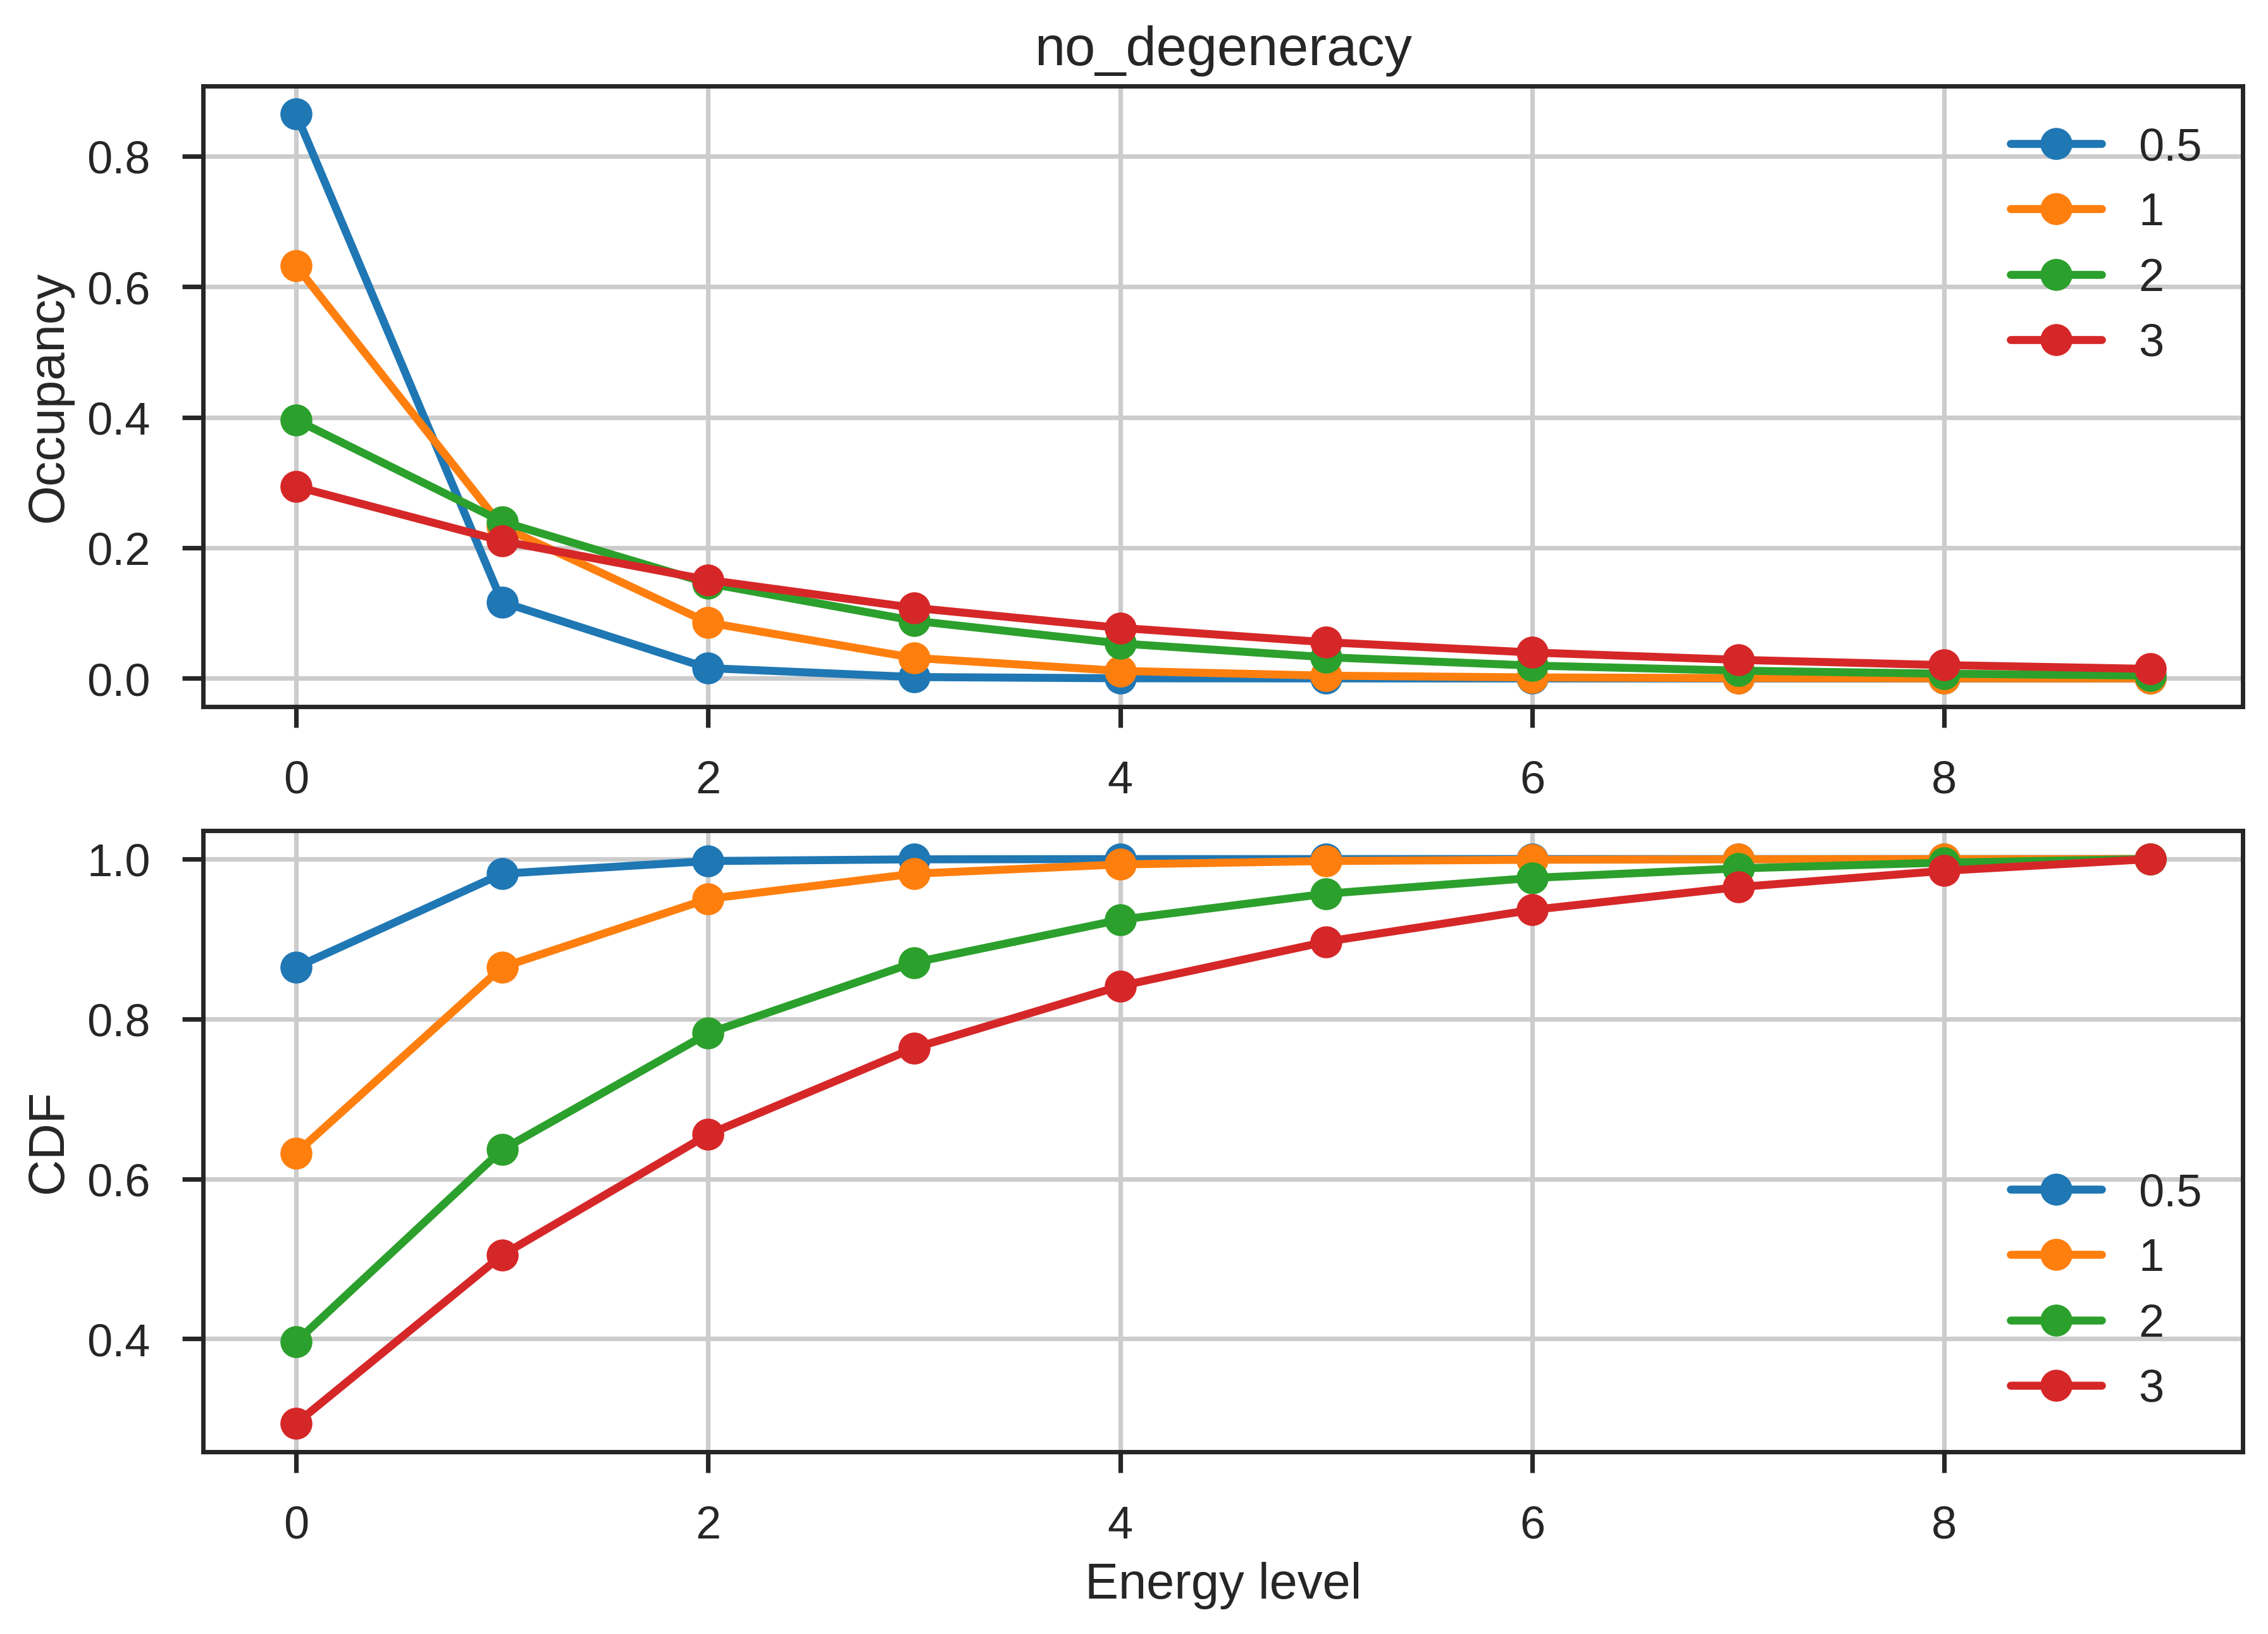
\includegraphics[width=0.8\linewidth]{noDegeneracy.png}		
			\caption{distribution with no degeneracy.}
			\label{fig::noDegeneracy}
		\end{figure}  
			
		We observe that the higher the temperature, the less the probability of finding a particle at a given energy level is. This is easier observed in the cumulative density function (CDF). When the temperature is low, we can say that the energy of our system is distributed more homogeneously. At temperature 1, we have that basically the probability of finding a particle at a fixed state is equal for all of such states. We cal also think of this as if the temperature is low, the particles are moving slowly. 
				
		\item
		Change the `calculateStateOccupancy()` function such that the degeneracies $(s + 1)$ and $(s + 2)$ are considered, where $s$ is the index of the energy level (use `numberOfEnergyLevels` = 10 and 		`reducedTemperature` = 0.5). Plot the results and include the graphs in your report. What can you infer from this trend? 
	
		\begin{figure}[H]
			\centering
			\begin{subfigure}[b]{0.7\linewidth}
				\centering
				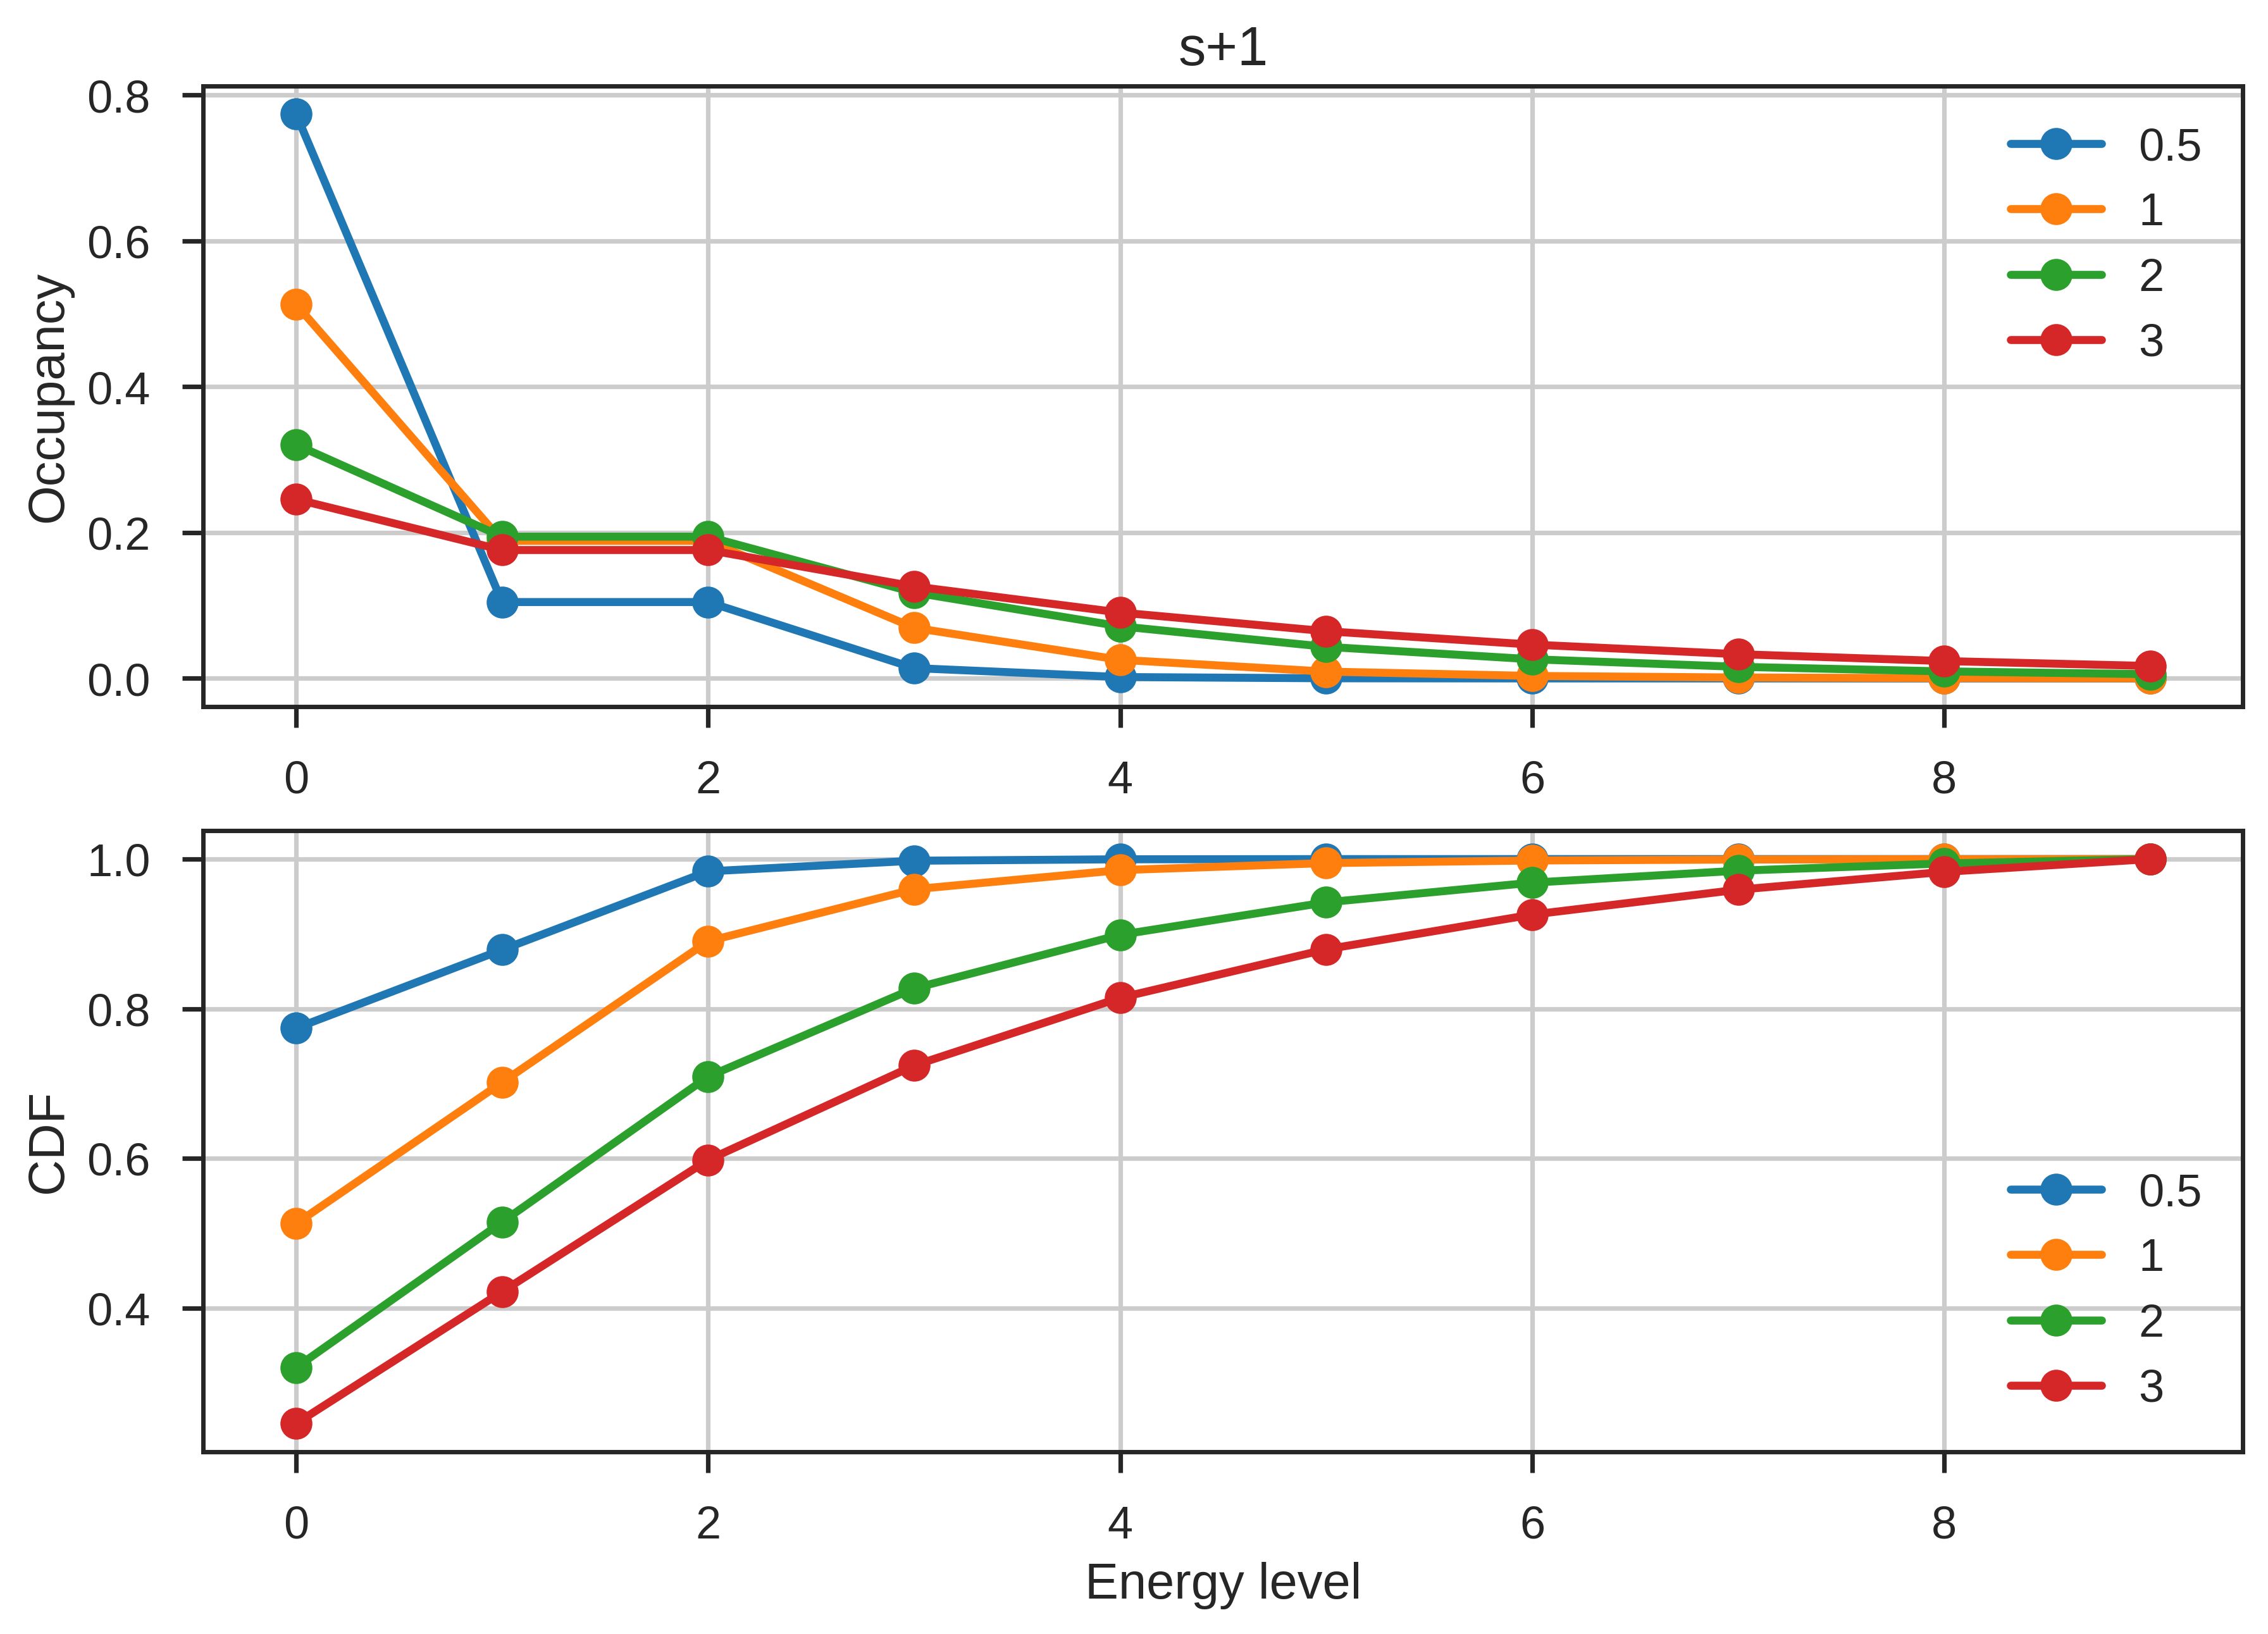
\includegraphics[width=0.8\linewidth]{degeneracy1.png}		
				\caption{Degeneracy s + 1.}
			\end{subfigure}		
			\hfill
			\begin{subfigure}[b]{0.7\linewidth}
				\centering
				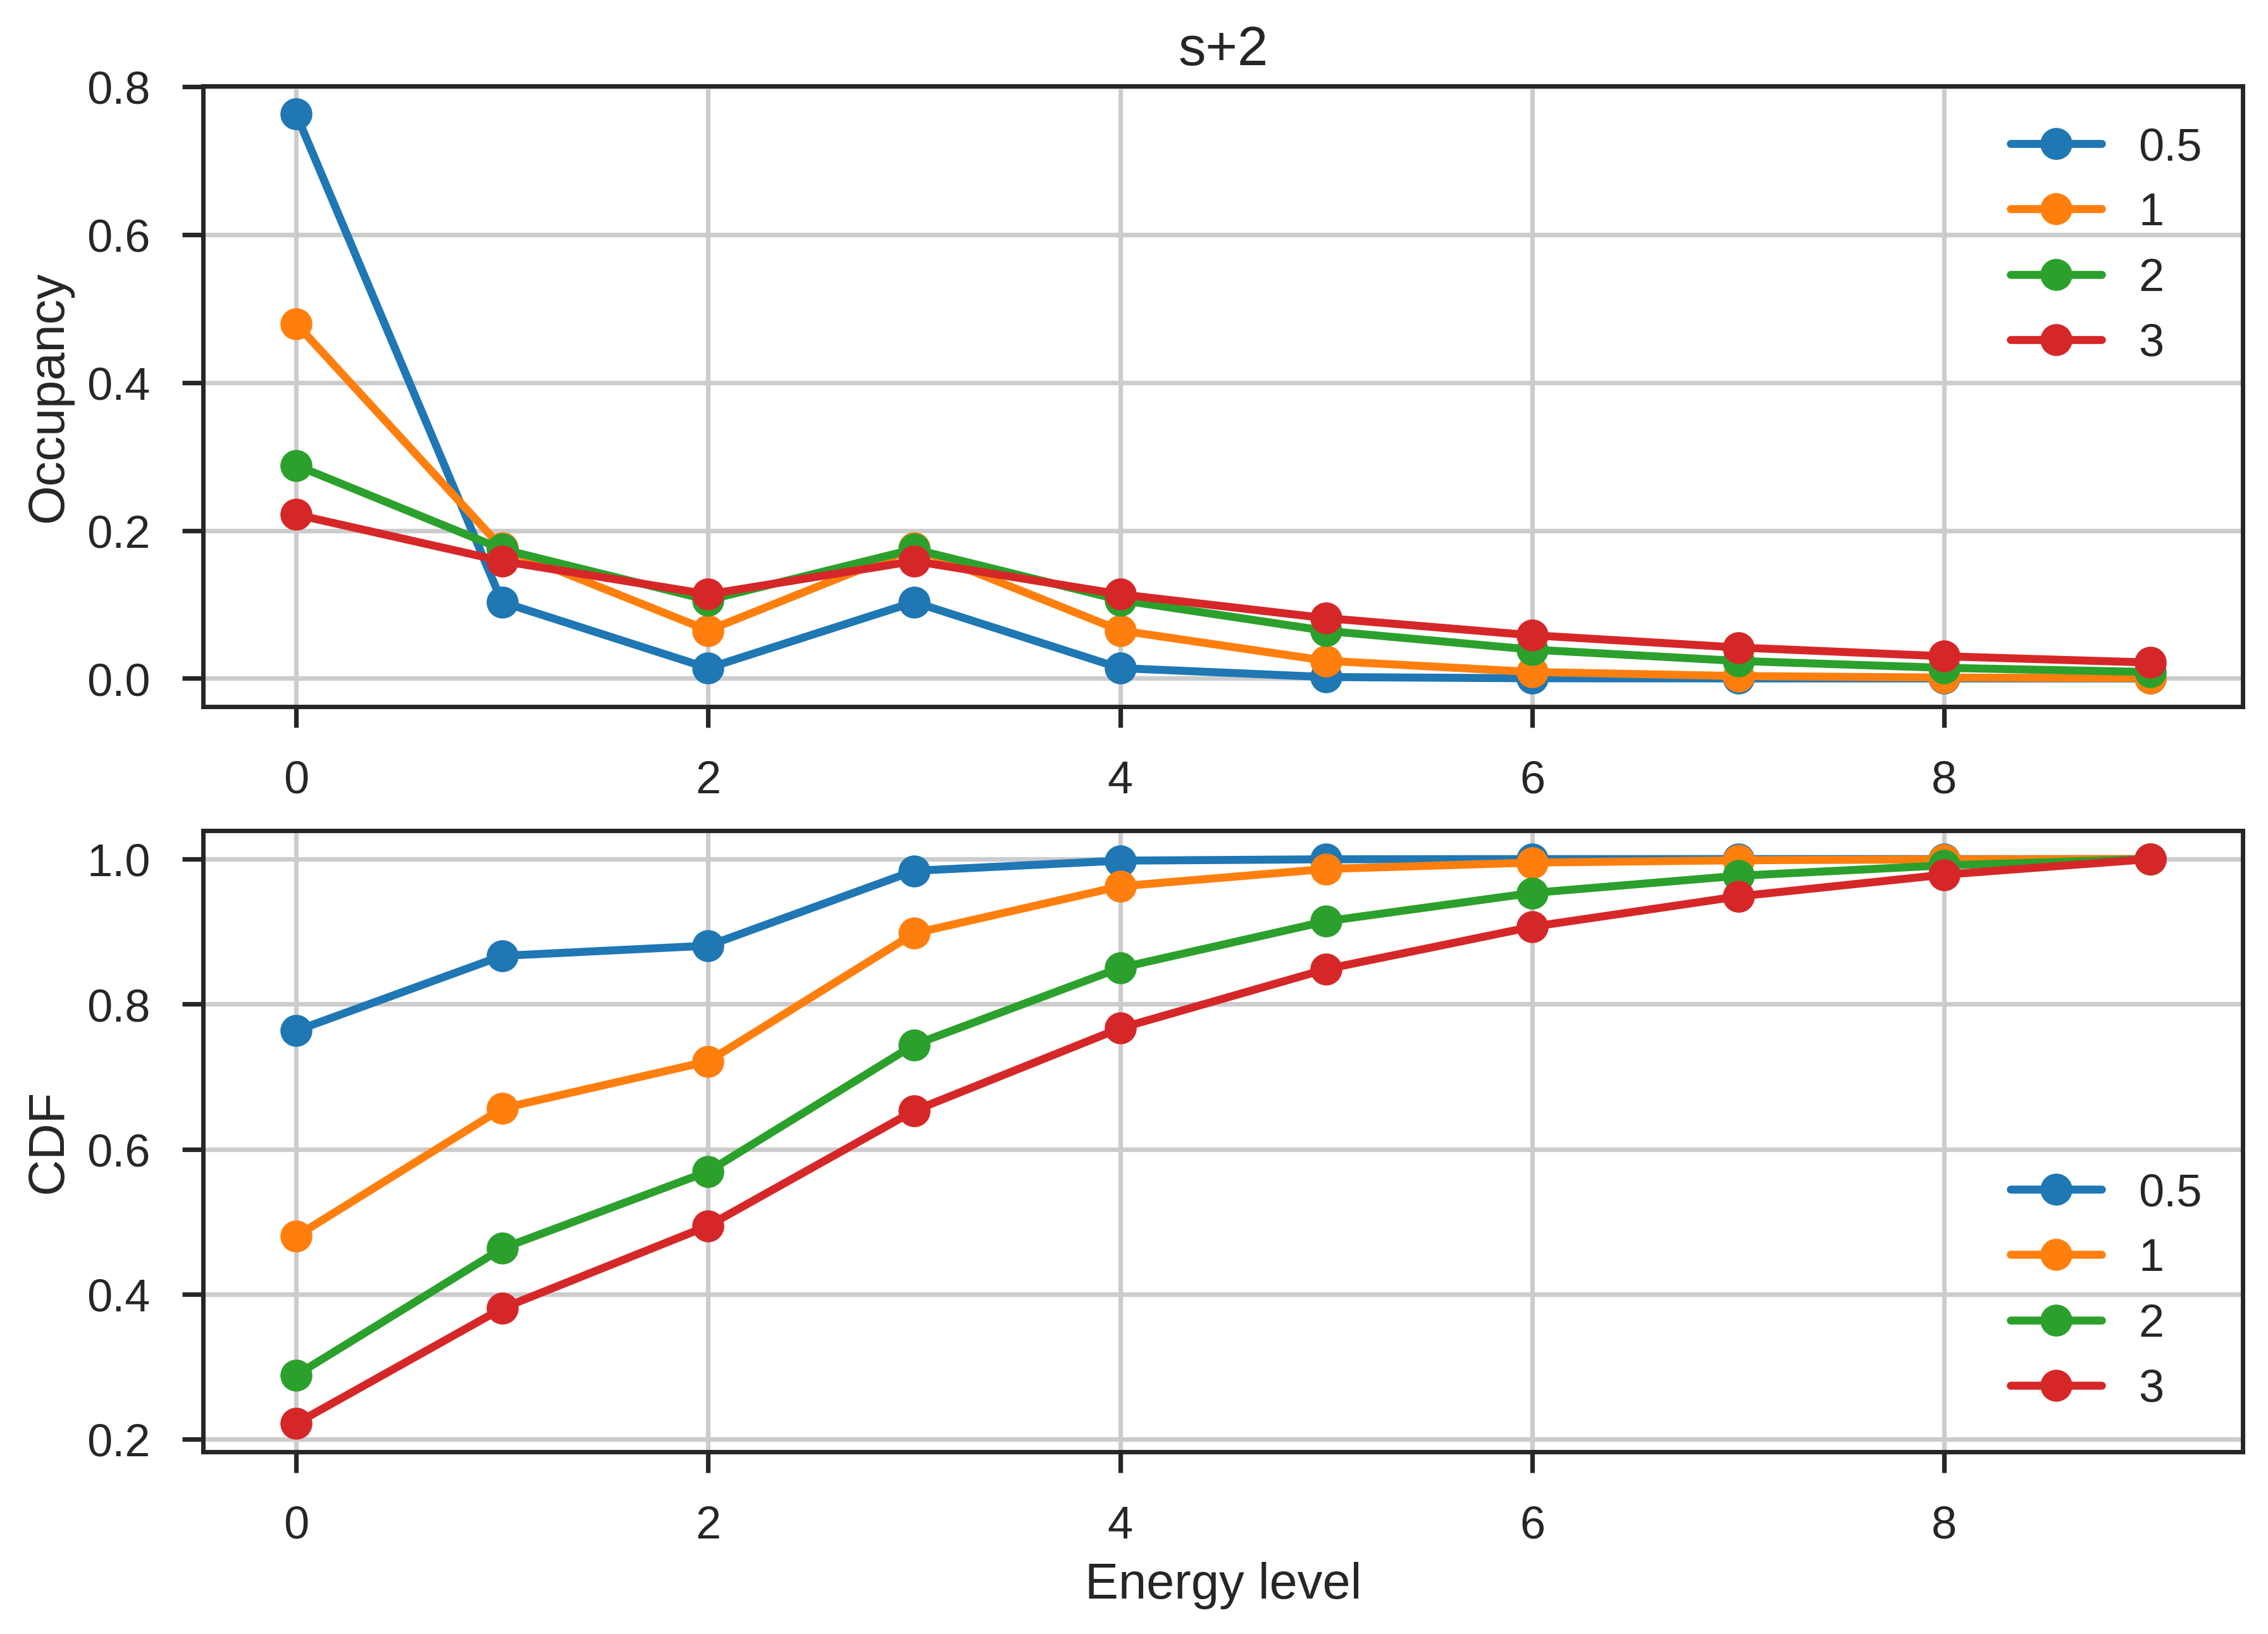
\includegraphics[width=0.80\linewidth]{degeneracy2.png}
				\caption{Degeneracy s + 2.}
			\end{subfigure}			
			\caption{Distribution for different degeneracies.}
			\label{fig::Degeneracy1}
		\end{figure}  	
		
		We observe something similar to the case with no degeneracy.
		
		\item
		Modify your program such that the state occupancy and partition	function are calculated for a linear rotor with moment of inertia 	$I$. Compare your results at different temperatures with the approximate result:
		
		$$
		Z = \frac{2I}{\beta\hbar^2}
		$$
		
		using
		
		$$
		\frac{I}{\hbar^2} = 1.
		$$
		
		Note that the energy levels of a linear rotor are:
		
		$$
		U = J(J+1)\frac{\hbar^2}{2I}
		$$
		
		with $J= 0, 1, 2, \dots, \infty$ and the degeneracy of level J is
		$2J +1$.		

		For the following plots, the code rotor.py was used: 
		
		\begin{figure}[H]
			\centering
			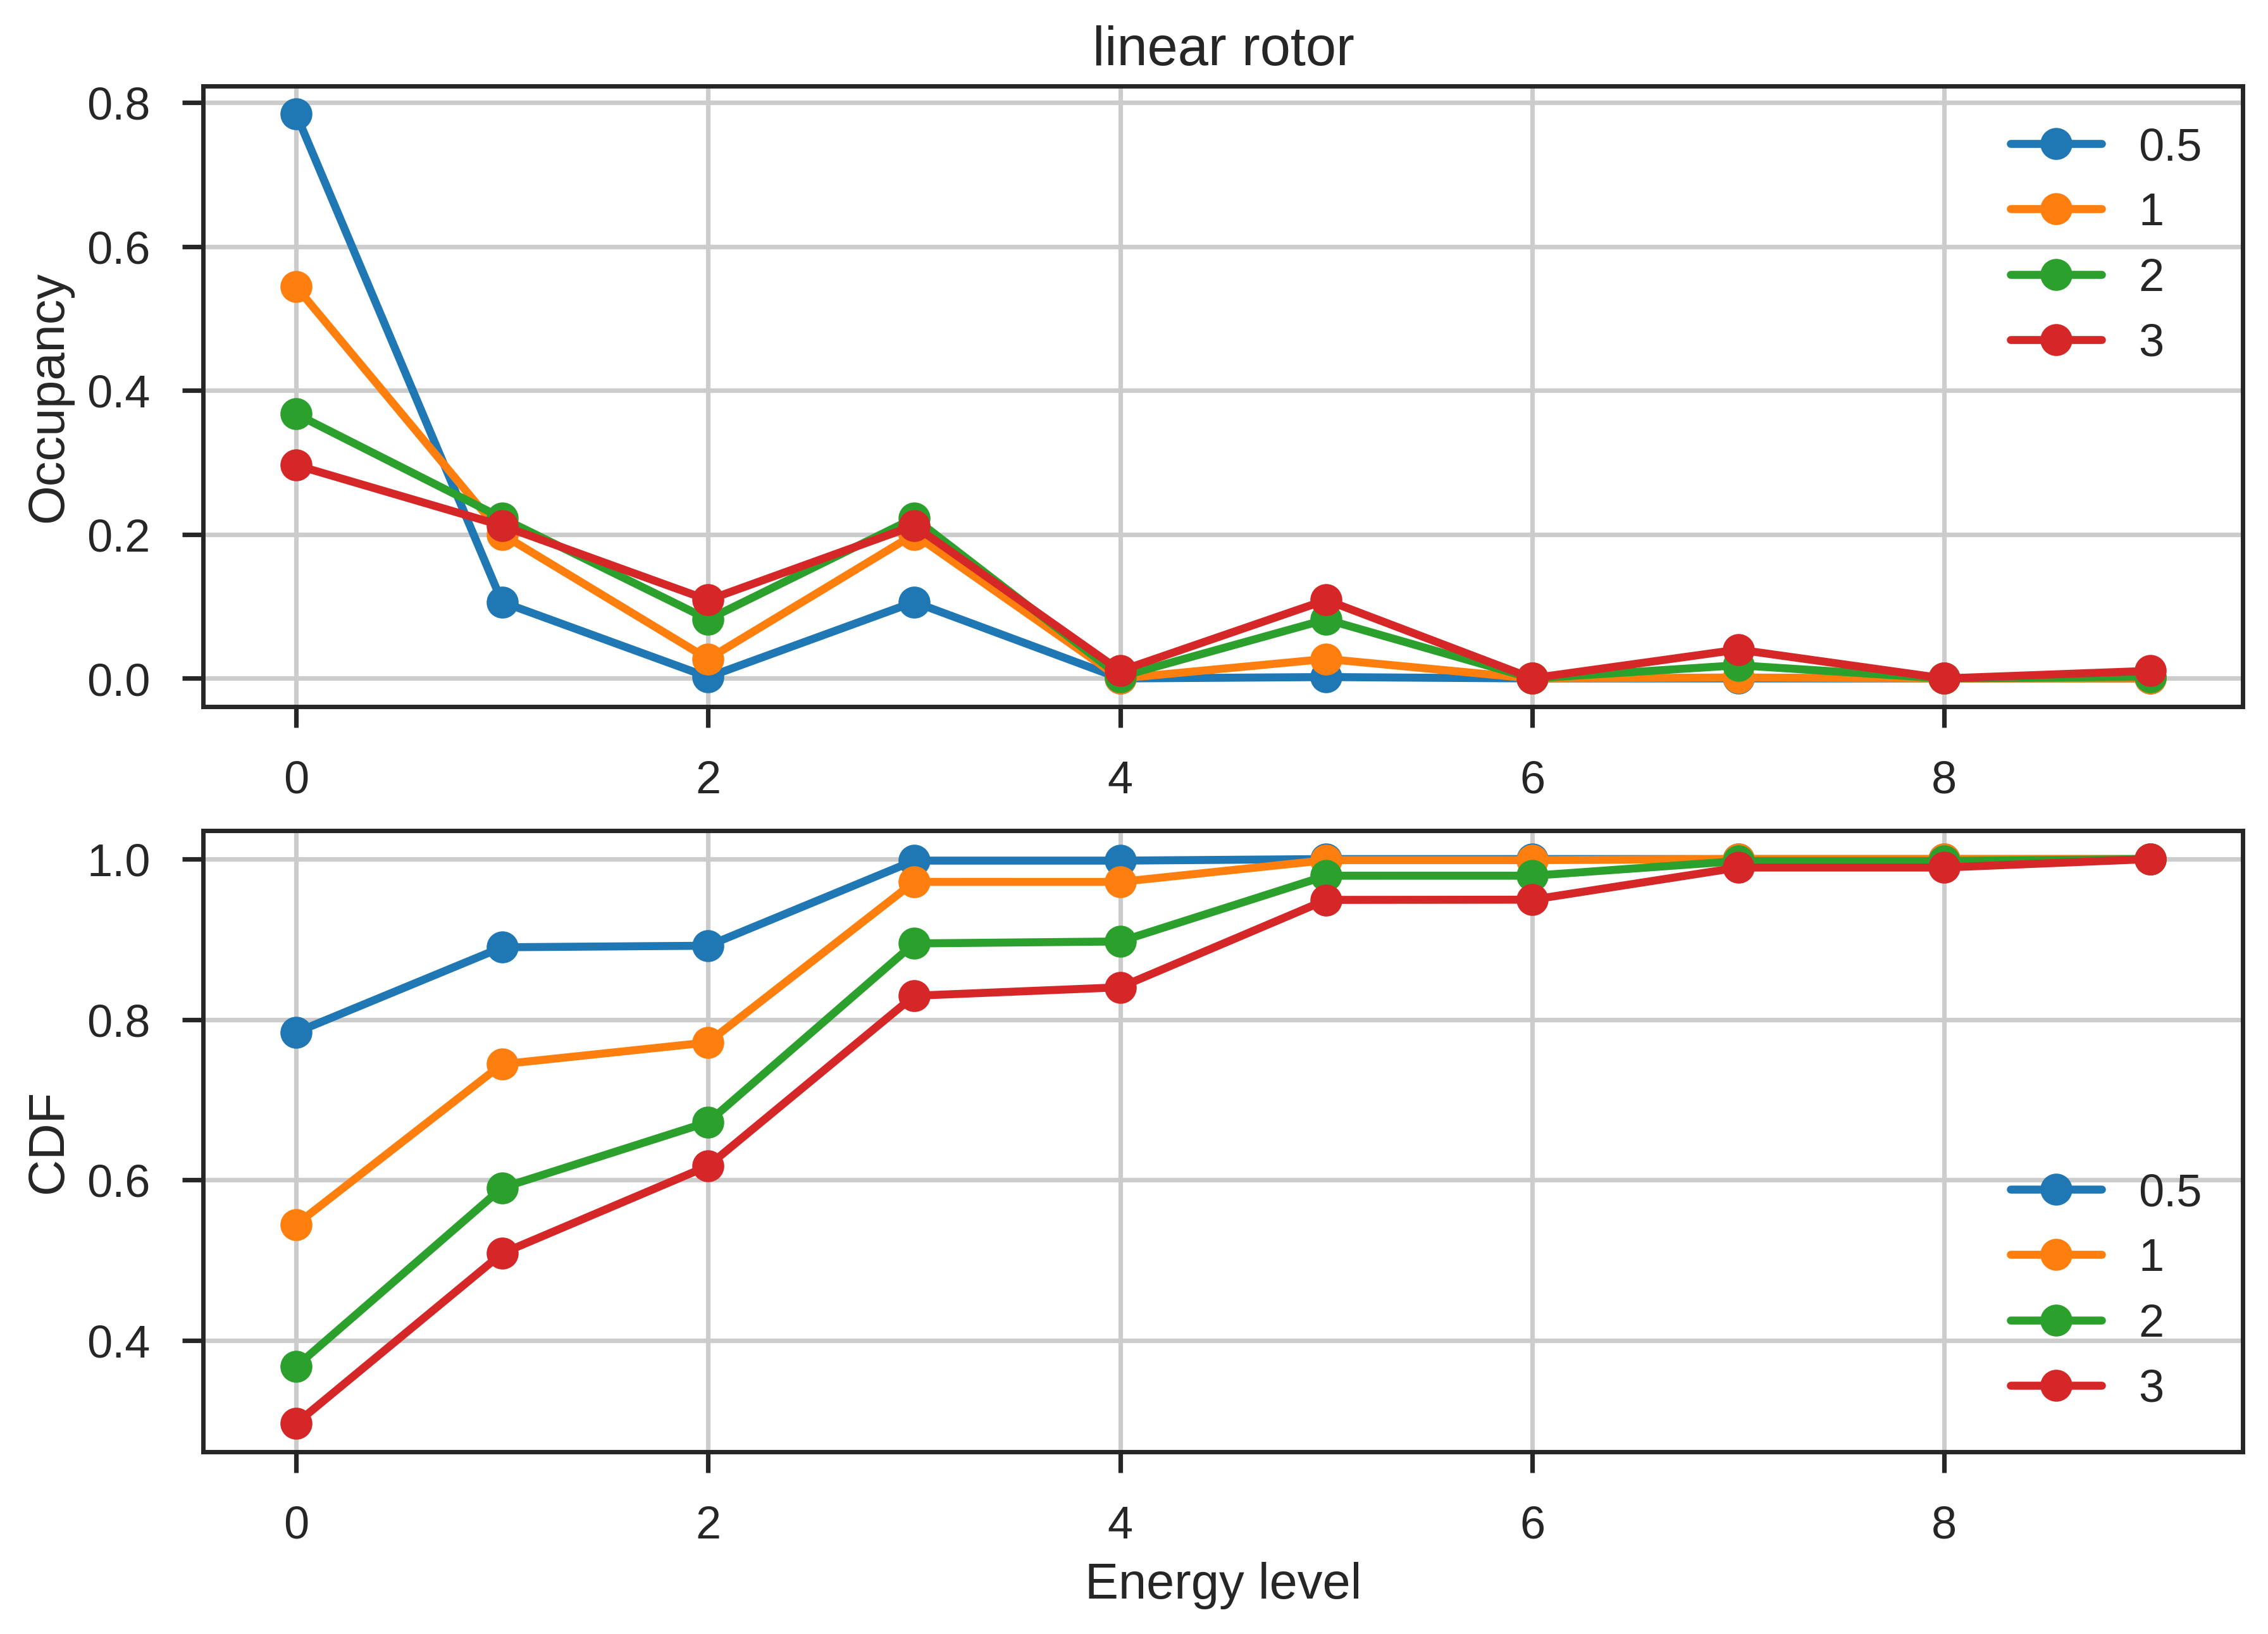
\includegraphics[width=0.8\linewidth]{rotor.png}		
			\caption{Linear rotor.}
			\label{fig::rotor}
		\end{figure}  
		
		We have that: 
		\begin{enumerate}
			\item 
			$Z_{computed,T_{1}} = 1.2756$ and $Z_{approximated,T_{1}} = 1$
			\item
			$Z_{computed,T_{2}} = 1.8379$ and $Z_{approximated,T_{2}} = 2$
			\item
			$Z_{computed,T_{3}} = 2.7226$ and $Z_{approximated,T_{3}} = 4$
			\item
			$Z_{computed,T_{4}} = 3.3764$ and $Z_{approximated,T_{4}} = 6$
		\end{enumerate}		
		
		Where $T_{1} =0.50$, $T_{2} =1$, $T_{3} =2$ and $T_{4} =3$.	We may say that the higher the temperature is, the less accurate our approximation to $Z$ is. 
		
		From the plots, we observe that the the higher the temperature is, find a particle at a given state of energy with is less probable since particles move much faster at higher temperatures.
		
		We note that since the denegeneracy is $2J+1$, if we take $J=1$, then the energy $E_{J=3}$ must equal to $E_{J=0}$, the energy $E_{J=5}$ corresponds to $E_{J=2}$, the energy $E_{J=7}$ corresponds to $E_{J=3}$, and so on. This means that the 'gap' between states with the same energy increases when $J$ increases.
		
	\end{enumerate}		
	
\end{document}    